% !TEX root = ../main.tex

% Project report section

\section{Project report}
\subsection{Background}
Bayesian Optimization (BayesOpt) is a framework to find the global optimum of expensive, black-box functions \cite{Frazier2018}. Originally from the computer experiments field, BayesOpt is often employed in machine learning, chemical engineering, materials sciences, and many other areas \cite{Garnett2023}. While multiple software implementations exist, here we focus on two popular choices: the BoTorch Python library \cite{Balandat2019} and the DiceOptim R package \cite{Roustant2012}.
\subsection{Methods}
The performance and efficiency of BayesOpt implementations were assessed using the Gap measure as defined in (\ref{gap}) and the time per iteration in seconds, respectively. The implementations compared were BoTorch (v. 0.10.0) and DiceOptim (v. 2.1.1) \cite{Roustant2012, Balandat2019}. Standardized versions of the Hartman 6 (H6), Rosenbrock 4 (Ros4), and Goldstein–Price (GP) test functions were implemented in Python following their validated R implementations in the DiceOptim and DiceKriging (v. 1.6.0) R packages\footnote{DiceKriging and DiceOptim were published together as complimentary R packages \cite{Roustant2012}.}. Specifically, the original functions were modified so that the input space ranged from 0 to 1 for all input dimensions. No validated implementation of the Shubert test function was available and, therefore, this test function was not used. All simulations employed noise-free observations of each test function.

Both BoTorch and DiceOptim implementations employed a Matérn kernel ($\nu=5/2$). Based 
on availability, Expected Improvement (EI), Knowledge Gradient (KG), and (log) Probability of Improvement (PI) were used as acquisition functions for BoTorch, and only EI and (approximate) KG were used for DiceOptim\footnote{Predictive Entropy Search was unavailable in both BoTorch and DiceOptim.}. Acquisition functions were optimized using the L-BFGS-B algorithm. The remaining parameters employed default values from each implementation.

A total of 100 simulation repetitions were run for each simulation scenario. Each simulation run consisted of an independent run of BayesOpt with a given set of implementation (BoTorch vs. DiceOptim), acquisition function (EI, KG, or PI), and test function (H6, Ros4, and GP). Within each run, an initial GP model was fit to $n_0=10$ observations of the corresponding test function, evaluated at points sampled uniformly at random from the input space; BayesOpt was then carried out for $n=30$ iterations. The relatively high $n_0$ was necessary to avoid numerical problems with DiceOptim, which employs Maximum Likelihood Estimation by default. The relatively low $n$ was chosen due to time limitations.

Finally, a ``negative control case'' was also assessed: instead of selecting the next evaluation point based on the acquisition function, we sample a point from the input space uniformly at random. This is intended as a minimal baseline to be outperformed by the actual BayesOpt methods.

All analyses are fully reproducible with as few as two commands with code from the GitHub repository \href{https://github.com/giulianonetto/qp-giulianonetto-bayesopt}{https://github.com/giulianonetto/qp-giulianonetto-bayesopt}, based on a fixed Docker image \cite{merkel2014} with Python (3.10) and R (v. 4.3.2).
\subsection{Results}
Gap and running time results were recorded across 100 simulation runs. The estimated mean Gap values per iteration are shown in Figure (\ref{fig:gap}). At a given iteration number, a higher mean Gap value means the optimization procedure reached closer to the global optimum, on average. Optimization performance varied substantially depending on test and acquisition functions as well as on the choice of implementation.

\begin{figure}[H]
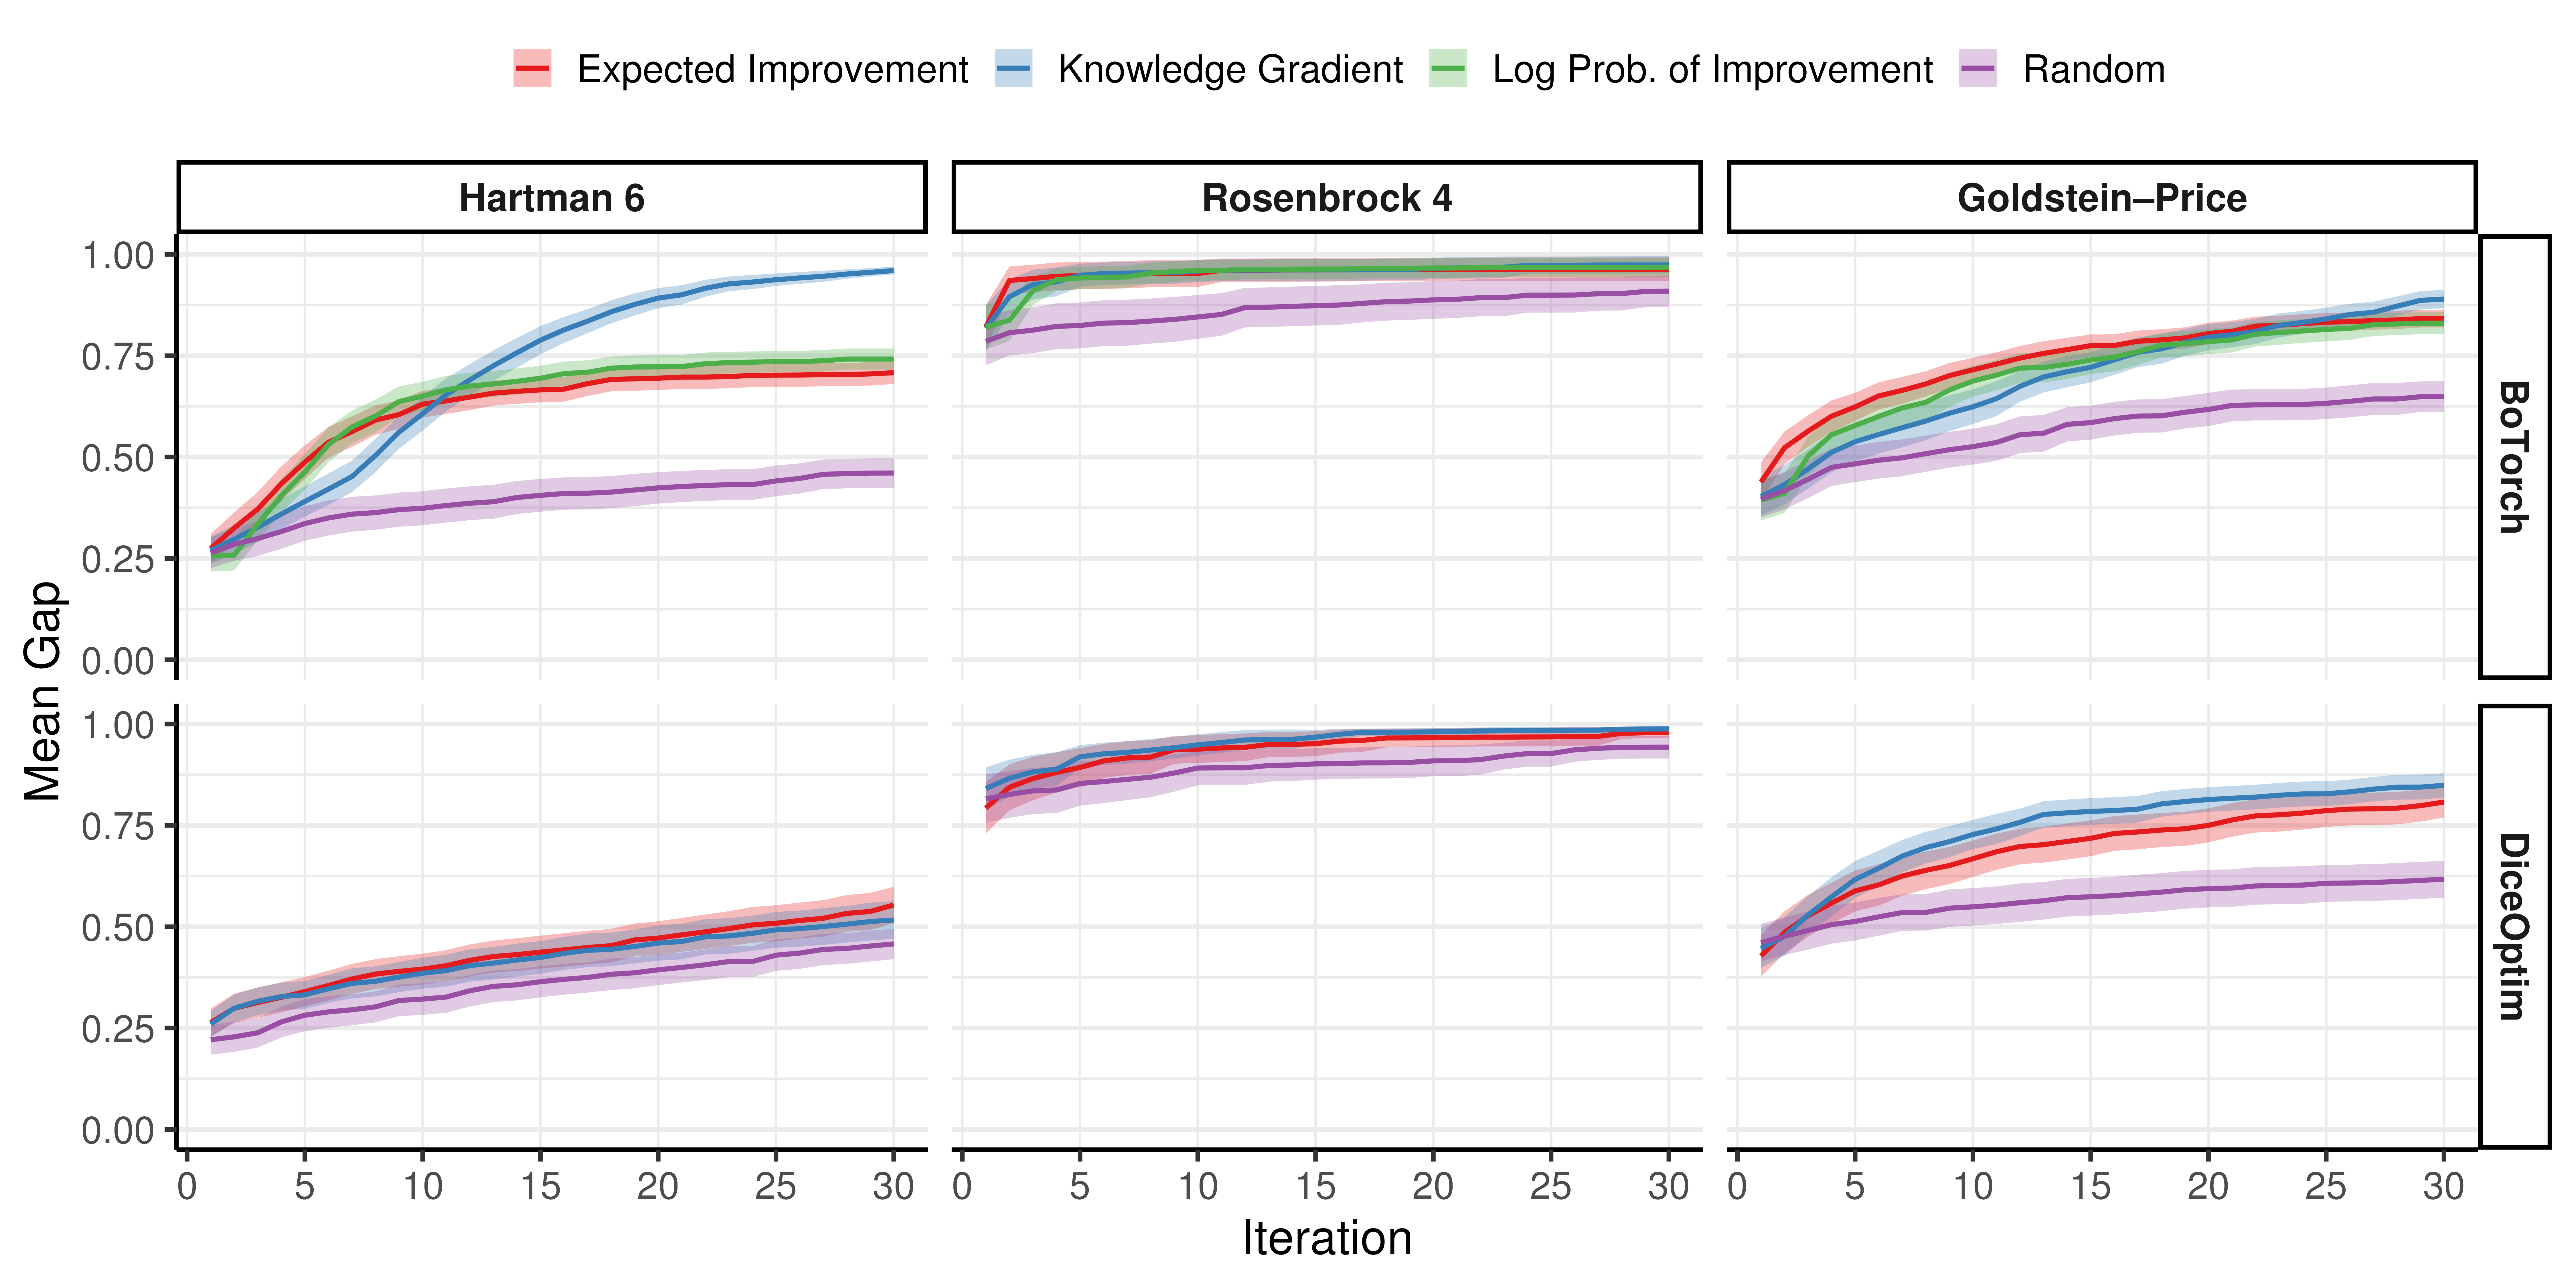
\includegraphics[width=0.99\linewidth]{output/gap_results.png}
\caption{\small \textbf{Optimization performance depends on test and acquisition functions as well as on implementation choice}. For each distribution, a two-group dataset with 1,000 features and either 5 or 50 samples per group was generated ($n=10$ and $n=100$, respectively). Points represent observed/theoretical quantiles of p-values from a two-sample t-test for each feature (theoretical distribution: Unif(0, 1)). Different colours indicate the proportion of the lowest overall mean features that were filtered out (e.g., ``Lowest 10\%" retains features whose overall mean is above the $10^{th}$ percentile of features' overall means). All features were sampled iid with the following distributions: Poisson($\lambda$=500), Binomial(n=1000, p=0.5), NB(size=$r_{\text{NB}}$, $\mu$=500), and Beta-Bin(size=$r_{\text{BB}}$, p=$0.5$, $\rho$=0.01). In the Negative Binomial and Beta-Binomial cases, the sizes $r_{\text{NB}}$ and $r_{\text{BB}}$ were sampled independently from a Poisson($\lambda$=1000) to emulate varying library sizes from NGS experiments. Dashed black lines represent the expected QQ line.}
\label{fig:gap}
\end{figure}

\subsection{Discussion}